\section{第一章\quad 绪论与基本概念}
\pt{工程热力学定义}：工程热力学是一门研究“热能有效利用”以及“热能和其他形式能量转换规律”的科学。
\pt{核心关注点}：热能如何转化为机械能，机械能如何服务于发电、推进、制冷、供暖等工程装置。
\pt{能源分类}：一次能源是天然存在、未经加工或转换的能源，如太阳能、天然气、石油、煤、水力、风能、地热、核能等\par
\noindent
\begin{minipage}[t]{0.62\linewidth}
  \vspace{0pt}
  \pt{热能动力装置}：从燃料燃烧或其他热源中获得热能，并利用热能得到动力的整套设备，包括燃气动力装置和蒸汽动力装置。
  
  内燃机、燃气轮机、喷气发动机等都属于典型热能动力装置。
\end{minipage}
\hfill
\begin{minipage}[t]{0.34\linewidth}
  \vspace{0pt}
  \centering
  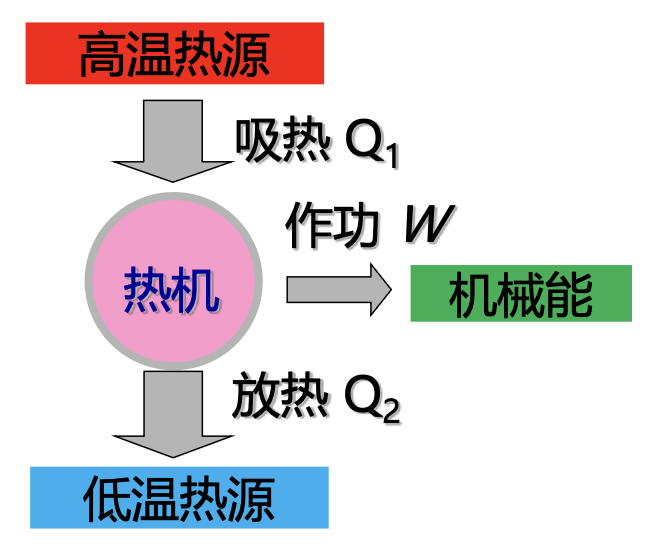
\includegraphics[width=.8\linewidth]{figures/1热机工作过程示意图.png}
  
  {热机过程}
\end{minipage}

\pt{工质}是实现热能和机械能相互转化的媒介物质,应具有\pt{适宜的膨胀性}、\pt{优良的流动性}、\pt{较大的热容量}、\pt{可靠的稳定性和安全性}、\pt{环境友好性}，并且\pt{价廉、容易大量获得}。\pt{热源}是工质从中吸取或向之排出热能的物质系统

\divider
\pt{热力系统}是\pt{人为分割}出来，作为热力学研究对象的有限物质系统
\pt{外界}是与体系发生质量、能量交换的物系
\pt{边界}是系统与外界的分界线
\pt{热力学系统的分类}
\begin{itemize}
  \item 按组元数分：
        \pt{单元系}：由单一纯物质组成，仅含有一种化学成分（\pt{分子种类相同}）；
        \pt{多元系}：系统由两种或以上组分组成，可以是混合物或溶液。
  \item 按相数分：
        \pt{单相系}：系统内所有物质处于\pt{同一相态}，宏观上没有界面分隔，可以是单元系也可以是多元系；
        \pt{复相系}：复相系内同时存在\pt{两种或以上相态}，相之间有\pt{明确界面}，各相性质不同。
  \item 按系统内部状态分：
        \pt{均匀系}：内部各部分物理性质和化学组成完全相同，温度、压力、密度、浓度等处处一致；
        \pt{非均匀系}：存在宏观界面，不同部分性质或组成有明显差异
  \item 按系统与外界质量交换分
        \pt{闭口系}：控制\pt{质量} CM，没有质量越过边界；
        \pt{开口系}：控制\pt{体积} CV，允许质量越过边界。
  \item 按能量交换分
        \pt{绝热系}：与外界没有热量交换，但是可以有功交换或者质量交换；
        \pt{孤立系 ISO}：与外界没有任何形式的质量或者能量交换。
  \item 简单可压缩系：由可压缩物质组成，如水蒸气、空气、燃气等；无化学反应；与外界交换容积变化功，是本课程中讨论的绝大部分系统。
\end{itemize}
这些分类不能简单等同：单元系未必均匀，例如气液平衡分离状态；复相系也未必宏观不均匀，例如湿蒸汽

\divider
\pt{热力学状态}是工质所呈现的宏观物理状况。\pt{状态参数}是描述工质状态的\pt{宏观}物理量；是大量分子运动的宏观平均效果，只有平衡态才有明确状态参数；是状态的单值函数，物理上与\pt{过程无关}，数学上\pt{其微量是全微分}，并且闭合积分为 $0$，$\oint\,\mathrm{x} = 0$。分为\pt{广延量}和\pt{强度量}两类，前者与系统质量成正比，后者与系统质量无关。

系统两个状态相同的充要条件是所有状态参数一一对应相等；对简单可压缩系，两个独立状态参数对应相等即可确定状态相同。

温度是物体冷热程度的标志，测温基础是\pt{热力学第零定律}，即若两个热力学系统均与第三个系统处于热平衡状态，此两个系统也必互相处于热平衡

$$
  \{t\}_{^\circ C}=\{t\}_K - 273.15
$$

\pt{压力}是单位面积上施加的垂直作用力，包括绝对压力 $p$、表压力 $p_\mathrm{e}$ 或 $p_\mathrm{g}$、真空度 $p_\mathrm{v}$、当地大气压 $p_\mathrm{b}$。当系统压力高于大气压：$p = p_\mathrm{b} + p_\mathrm{e}$。当系统压力低于大气压：$p = p_\mathrm{b} - p_\mathrm{v}$。

比体积是单位质量工质的体积：$v = \frac{V}{M}$，单位 $m^3/kg$，密度是单位体积工质的质量：$\rho = \frac{M}{V}$，单位 $kg/m^3$，两者互为倒数：$v = \frac{1}{\rho}$。

\divider
\vspace{0pt}
\pt{热力学过程}是系统状态发生变化的过程，分为\pt{平衡过程}和\pt{非平衡过程}两类。前者系统始终处于热力学平衡态，后者系统至少存在一个状态参数不均匀分布或者存在不可逆现象。

\pt{热力学循环}是系统经历一系列状态变化后回到初始状态的过程。


\pt{热力学能} $U$ 是状态参数，单位为 $J$，一般情况下可写成 $U=U(T,v)$，微分形式为 $\mathrm{d}U=\left(\frac{\partial U}{\partial T}\right)_V\mathrm{d}T+\left(\frac{\partial U}{\partial V}\right)_T\mathrm{d}V=c_V\mathrm{d}T+\left[T\left(\frac{\partial p}{\partial T}\right)_V-p\right]\mathrm{d}V$

\begin{center}
  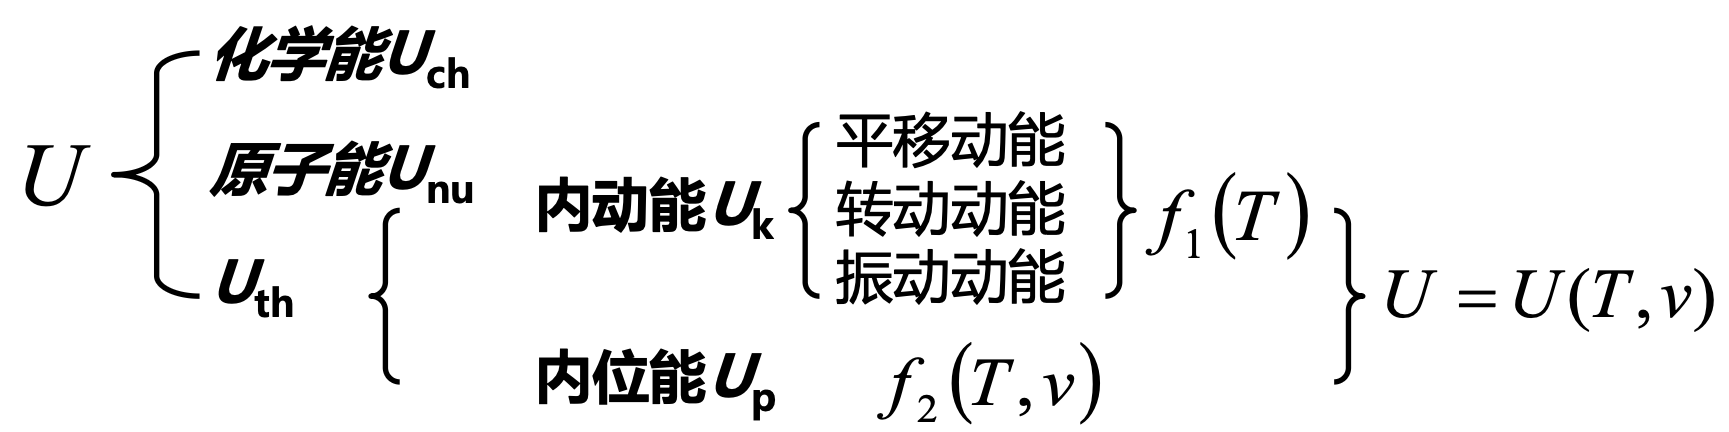
\includegraphics[width=\linewidth]{figures/1热力学能组成.png}
  
  {热力学能的组成}
\end{center}

\pt{总（储存）能}包括热力学能、宏观动能和宏观位能 $E=U+E_k+E_p$

\divider
\pt{推动功}是系统引进或排除工质传递的能量，系统引进或排除工质时，由压力作用产生的功 $W = pV$ \newline
\pt{流动功}是系统维持工质流动所需要的功，常表示为 $pv$，体现单位质量工质的流动功
\pt{焓}为 $H=U+PV$，$\mathrm{d}H=c_p\ \mathrm{d}T+\left[v-T\left(\frac{\partial V}{\partial T}\right)_p\right]\ \mathrm{d}p$\newline
\pt{平衡状态}是热力系统在不受外界影响条件下，状态参数不随时间改变的状态。系统达到平衡的充要条件是系统同时达到\pt{热平衡}和\pt{力平衡}
\pt{热平衡}为无外界作用下热力系统各部分之间没有热量的传递，系统内部、系统与外界处处\pt{温度相等}；
\pt{力平衡}为无外界作用下，系统各部分之间没有相对位移，系统内部、系统与外界处处\pt{压力相等}。
\pt{状态方程}为 $f(p,V,T)=0$

\divider
\pt{准静态过程}为偏离平衡态无穷小，随时恢复平衡的状态变化过程，可在状态参数图上用连续实线表示。进行条件为坏平衡的\pt{势差无穷小}；过程进行无限\pt{缓慢}；工质具有\pt{恢复平衡}的能力。\newline
\pt{可逆过程}为系统可\pt{经原途径返回原来状态}而\pt{在外界不留下任何变化}的过程。可逆过程为\pt{无耗散效应}的\pt{准静态过程}。

\divider
